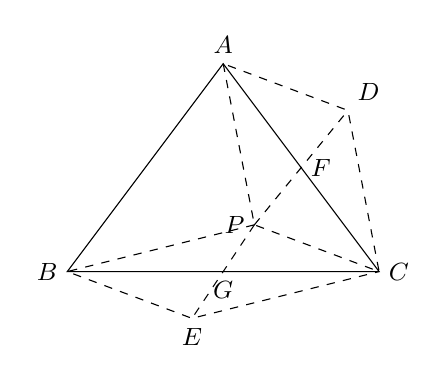
\begin{tikzpicture}[scale=.66, every node/.style={font=\small}]
  \coordinate (A) at (0,4); \coordinate (B) at (-3,0); \coordinate (C) at (3,0);
  \coordinate (P) at (.60,.90); \coordinate (D) at (2.40,3.10); \coordinate (E) at (-.60,-.90);
  \coordinate (F) at (1.50,2.00); \coordinate (G) at (0,0);
  \draw (A)--(B)--(C)--cycle;
  \draw[dashed] (A)--(P)--(C)--(D)--cycle;
  \draw[dashed] (P)--(B)--(E)--(C);
  \draw[dashed] (P)--(D) (P)--(E);
  \foreach \p/\pos in {A/above,B/left,C/right,D/above right,E/below,F/right,G/below,P/left}
    \node[\pos] at (\p) {$\p$};
\end{tikzpicture}
